% +--------------------------------------------------------------------+
% | Sample Chapter
% |
% | This file provides examples of how to
% | - insert a figure with a caption
% | - construct a table with a caption
% | - create subsections within the chapter
% | - insert a reference to a Figure or Table
% | - make a citation
% +--------------------------------------------------------------------+

\cleardoublepage

% +--------------------------------------------------------------------+
% | Replace "Chapter Title" below with the title of your chapter.  LaTeX
% | will automatically number the chapters.
% +--------------------------------------------------------------------+

\chapter{Introducción}
%\label{ch:chapter1}
\label{makereference}

Entre los años 2008 y 2009 comenzaron a usar el concepto Internet de las cosas (abreviado IoT) como una apuesta hacia el futuro, cuyo objetivo era interconectar dispositivos digitales a internet.

Esto ya es una realidad, con mayor frecuencia encontramos nuevos dispositivos capaces de conectarse a internet, permitiendo al usuario su manejo desde cualquier parte del mundo. Con ello se abre camino a nuevas oportunidades haciendo la vida más cómoda al usuario y proporcionándole mayor seguridad y control.

Según empresas del sector tecnológico, en 2016 se espera que haya más de 6.000 millones de dispositivos basados en este concepto.

El concepto del internet de las cosas agrupa múltiples capacidades, algunas de ellas han sido utilizadas en el proyecto, estas se nombran a continuación:

\textbf{Comunicación y cooperación:} Dispositivos capaces de conectarse a la red de internet y entre ellos, intercambiando datos y comunicándose con servidores.

\textbf{Direccionamiento:} Los objetos serán localizables y configurables desde cualquier lugar de la red de internet.

\textbf{Identificación:} Los objetos se identificarán en la red por medio de tecnologías como RFID (Radio Frecuency Identification), códigos de barras ópticos, NFC (Near Field Communication) y otras muchas formas.

\textbf{Localización:} Se podrá saber la ubicación física del dispositivo en cualquier momento.

El proyecto nace con el objetivo de emprender en esta tecnología, para ello se quiere conectar entre sí un sensor de acelerometría y un microprocesador para recibir y procesar sus datos. Dicho microprocesador debe estar provisto de Bluetooth de Bajo Consumo (en inglés, Bluetooth Low Energy o BLE) para poder enviar los datos vía Bluetooth a una aplicación móvil desarrollada en Android creada por los alumnos.

Existe una amplia variedad de dispositivos de bajo coste que podrían considerarse, ya que el mercado de los microprocesadores de bajo consumo está ahora en expansión y hay gran oferta de estos dispositivos, con entornos de desarrollo que ofrecen distintas alternativas y que previsiblemente irán reduciéndose en los próximos años cuando predomine una tecnología que se imponga a las demás.

Unas de las  empresas más especializadas en este tipo de tecnologías y que resaltan en este mercado son \textbf{Nordic Semiconductor, Cypress Semiconductor, Texas Instruments (TI), Cambridge Silicon Radio (CSR)} y \textbf{Dialog Semiconductor}.

Destacamos 2 empresas que nos han ofrecido mejores soluciones de microprocesadores de bajo consumo según las necesidades del proyecto:

\textbf{Nordic} está a la vanguardia de la revolución inalámbrica y son especialistas en Radiofrecuencia de consumo ultra bajo (ULP) redefiniendo nuevos procesadores por su bajo consumo, precios competitivos y aumentando la potencia de estos.
Esta empresa de semiconductores integra procesadores basados en la arquitectura ARM de 32 y 64 bits que predominan en el mercado de la electrónica. Son procesadores relativamente simples siendo ideales para aplicaciones de bajo consumo y tiene un precio económico. 

\textbf{Cypress} es una empresa especializada en ofrecer soluciones de alta calidad para sistemas integrados en el sector aeroespacial, automoción, industria, redes, telecomunicaciones y electrónica de consumo, entre otros campos. Cubre una amplia gama de productos entre los cuales destacan los microprocesadores, memorias,  sistemas programables en chips , lo que denominan (en inglés Programable System on Chip o PSOC), controladores táctiles capacitivos y controladores inalámbricos Bluetooth de bajo consumo

\section{Entornos de desarrollo}
\label{makereference1.1}

Con los dispositivos de bajo consumo nacen también multitud de entornos de desarrollo específicos para desarrollar todo su potencial, lo que dificulta la exploración de hardware, pues es necesario trabajar con un nuevo entorno cada vez. 

mbed, creada por la empresa ARM, es una plataforma de desarrollo \textit{online} que intenta hacer frente a esta variedad de entornos facilitando el desarrollo de prototipos de sistemas basados en microprocesadores.

Esta plataforma se creó para promover el Internet de las Cosas (IoT) y desarrollar proyectos mediante herramientas de construcción de hardware y software que aceleren el desarrollo de dispositivos basados en ARM.

Su enfoque está basado en la \textit{nube} y permite codificar, añadir librerías y compilar desde un navegador web. La ventaja de programar desde cualquier navegador es que permite tener accesibilidad desde cualquier punto del mundo sólo con conexión a internet. Durante el Capítulo~\ref{makereference4} se explicará con más detalle este entorno y cómo nos ha ayudado a llevar a cabo este proyecto.

Todo lo anterior hace de la compatibilidad con mbed una característica atractiva a la hora de elegir un dispositivo para llevar a cabo nuestro proyecto, lo que nos ha ayudado a elegir la placa de desarrollo nRF51-DK de Nordic.

\section{Bluetooth Smart: Bluetooth de bajo consumo}
\label{makereference1.2}

Uno de los rasgos fundamentales de IoT es la conectividad. Para lograrla tenemos a nuestra disposición una gran variedad de tecnologías inalámbricas, entre ellas \textit{zygbee}, \textit{narrow-band} o \textit{WiFi}; pero la que sin duda alguna ofrece el menor consumo de energía posible es \textit{Bluetooth Low Energy} (BLE, también denominado \textit{Bluetooth Smart}). 
Esta tecnología nace del Bluetooth clásico, pero marca su propio camino al sacrificar ancho de banda y períodos de envío continuados para lograr la meta de ser muy eficiente energéticamente, lo que lo hace perfecto para dispositivos que necesitan funcionar con una batería pequeña durante largos períodos. El hecho de ser parte de Bluetooth y poderse complementar con él hace que actualmente esté presente en todos los teléfonos móviles del mercado. A esto ayuda que grandes empresas del mundo de la tecnología y las telecomunicaciones respalden BLE.

En el Capítulo~\ref{makereference2} hablaremos de cómo se estructura e implementa Bluetooth Low Energy. 

\section{Especificación del objetivo del proyecto}
\label{makereference1.3}

El objetivo de este proyecto consiste en medir el esfuerzo realizado por un ciclista durante un trayecto. Esto se consigue combinando los valores proporcionados por un acelerómetro y los datos de posicionamiento por GPS para poder elaborar un mapa del trayecto en el que se indiquen las zonas que, por pendiente, estado del terreno, etc. supusieron un mayor esfuerzo. Además se ofrecerá más información que pueda ser calculada con estos datos, como la velocidad media o la distancia total recorrida, por ejemplo.

Para la comodidad del usuario, toda la información de la ruta se recogerá en su dispositivo móvil, del que se obtendrán los datos de localización y que se conectará a través de Bluetooth Smart con el sensor de acelerometría. De este modo, con un simple gesto podrá visualizar fácilmente los datos más relevantes.

\begin{figure}[h]%t=top, b=bottom, h=here
	\centering
    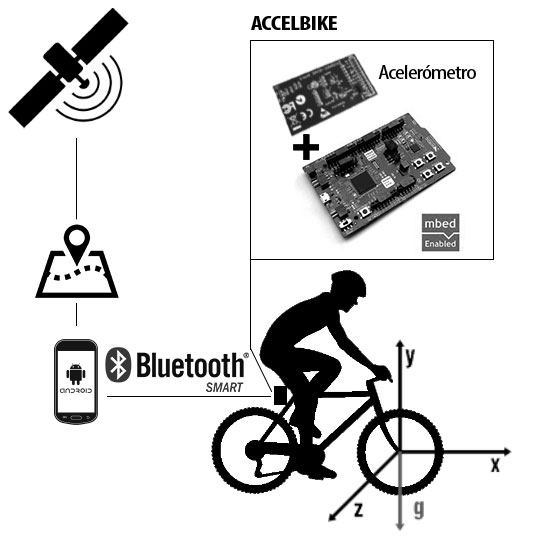
\includegraphics[scale=0.5]{figures/esquema_accelbike.jpg}
    \caption[Esquema del funcionamiento del proyecto]{Esquema del funcionamiento del proyecto. El dispositivo móvil recoge datos tanto de la localización como de un sensor de acelerometría.}
   	\label{figuraEsquemaAccelbike}
\end{figure}

\newpage % Esto esta aqui para que la imagen anterior no se meta dentro de las contribuciones

\section{Contribuciones Personales}
\label{makereference1.4}

\subsection{Rodrigo Claudio Miguez Rein}

La tarea principal que he realizado durante este proyecto es la de la programación de la placa nRF51-DK de Nordic para configurar la recepción de las muestras de acelerometría utilizando el bus de datos I2C y el envío de éstas por medio de la tecnología Bluetooth Low Energy.

En cuanto elegimos este proyecto, empecé a recopilar información junto con mis compañeros sobre las distintas soluciones \textit{System on Chip} con Bluetooth Smart integrado disponibles en el mercado. Para ello me informé sobre las tecnologías disponibles para realizar la conexión con un acelerómetro y sobre qué características necesitábamos en términos de procesamiento, memoria RAM y flash.

Durante este periodo también comencé a investigar sobre el funcionamiento y las características de Bluetooth Low Energy, buscando material de referencia para aprender todo lo posible sobre ésta.\\

Una vez escogimos dos placas de desarrollo, el kit CY8CKIT-042-BLE de la empresa Cypress Semiconductor y el modelo nRF51-DK de Nordic Semiconductor, comenzamos la fase de pruebas para familiarizarnos con las tecnologías que íbamos a usar. En mi caso, realicé las pruebas con la placa de Cypress. Para ello busqué tutoriales en la página web oficial de la empresa~\cite{CypressTutorials} y encontré un repositorio en GitHub con 100 proyectos de ejemplo~\cite{100Projects} que me ayudaron en gran medida para entender la programación del kit y los métodos para utilizar Bluetooth Low Energy y para realizar la comunicación con otros dispositivos. Descargué la aplicación móvil \textit{CySmart}, que permite probar los códigos de ejemplo, con una interfaz limpia y clara, que además ofrece su código fuente, lo que me sirvió para comprobar cómo se realiza el enlace por Bluetooth Low Energy en el lado de Android.
Entre los ejemplos disponibles para esta placa se encuentra: un sistema de alerta, que consiste en el envío de una señal al dispositivo para apagar o encender un LED y para hacer que parpadee, una aplicación de sensor de proximidad, que aprovecha un circuito integrado en la placa de desarrollo diseñado para este fin, enviando el valor recogido por el sensor al móvil, donde, con la aplicación CySmart mencionada anteriormente, se puede visualizar como una escala.

Durante la fase de pruebas realicé el código que permitía al CY8CKIT-042-BLE leer por SPI los datos recogidos de un circuito, consistente en un conversor analógico-digital contectado a una fotoresistencia, y enviarlos por Bluetooth Low Energy a una aplicación de prueba realizada en Android. Seguidamente comencé con las pruebas para recibir por I2C los datos del acelerómetro. Estas pruebas se detallarán más adelante en esta memoria.

Cuando elegimos la placa de Nordic, escogí continuar la parte del proyecto que se centraba en la programación de ésta, ya que me había resultado muy interesante la experiencia con el kit de Cypress. Realicé la conexión por I2C de Xtrinsic Sense-Board, una placa que contiene un chip de acelerometría. Para ello busqué su \textit{datasheet}~\cite{DatasheetAcc} para saber qué pines utilizaba, de qué manera recolectaba las muestras y cómo había que realizar la comunicación entre nRF51-DK y este periférico para lograr una transmisión correcta de los datos. Una vez pude comprobar que se recibía la información de acelerometría, elaboré un sistema para filtrar el ruido presente en las muestras y realicé la configuración de la placa de Nordic para que las transmitiera utilizando Bluetooth Low Energy.

En la parte de la aplicación Android, ayudé con el diseño de las clases que se iban a utilizar elaborando diagramas, y proporcioné \textit{feedback} a mis compañeros para hacerles saber en qué formato se iba a mandar la información por Bluetooth para que pudieran configurar en consecuencia la recepción en el móvil. 

\subsection{David Muñoz Lorenzo}

\subsection{Alexis Vizcaya Hervella}

%\begin{figure}[htb]%t=top, b=bottom, h=here
%
%    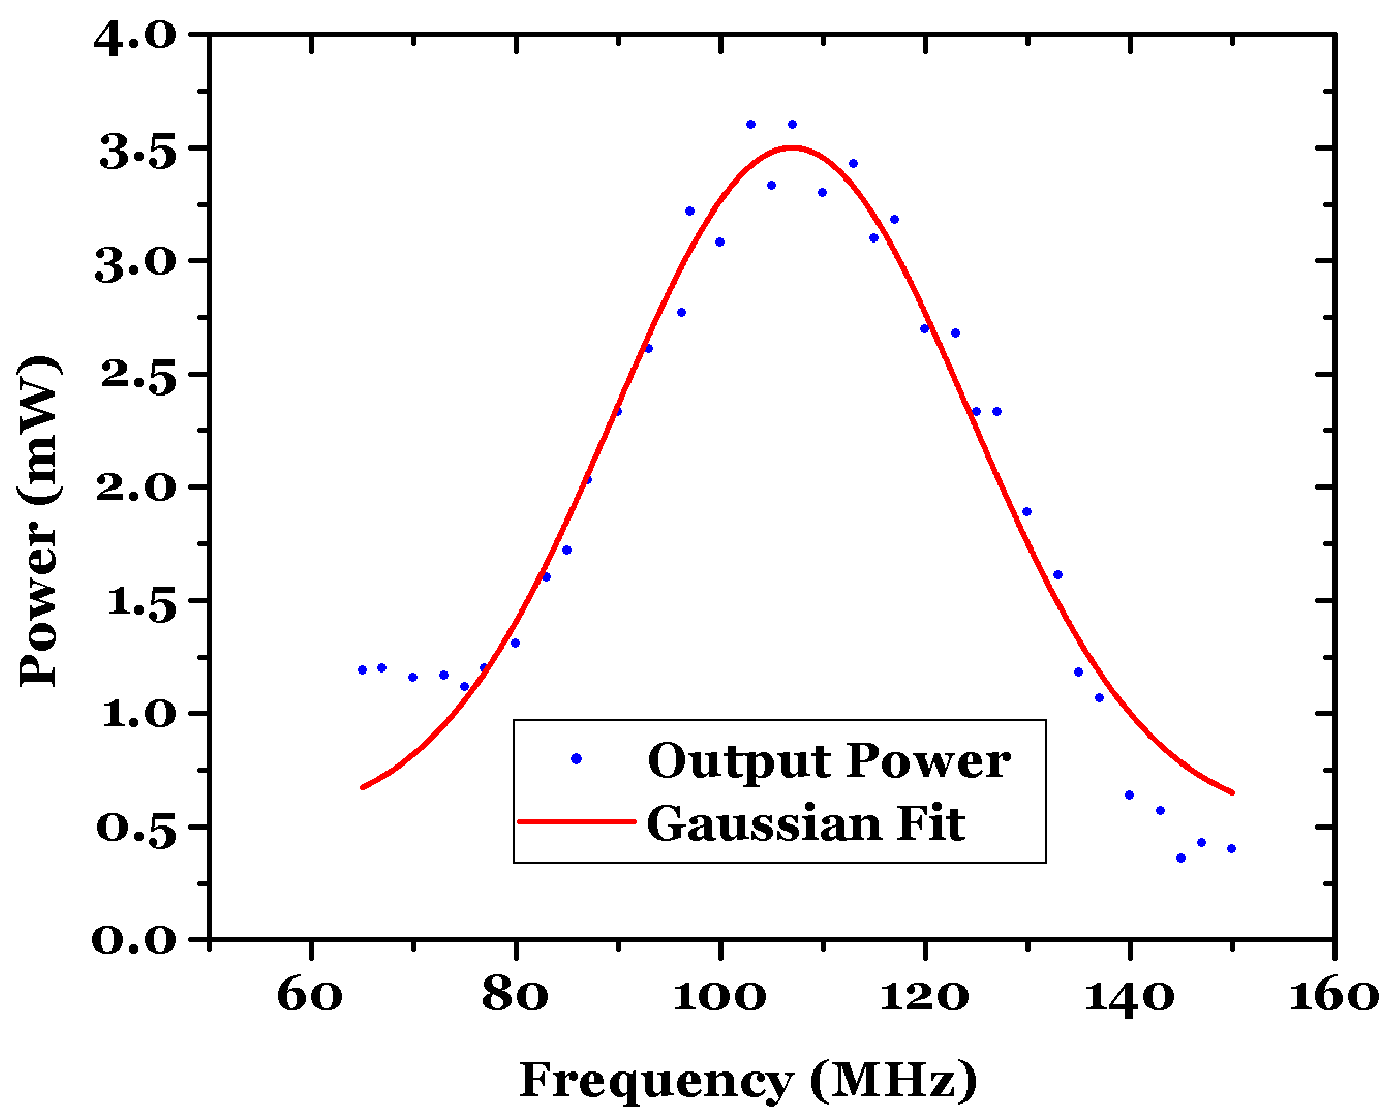
\includegraphics[height=2.5in]{figures/graph.png}
%
%    \caption[Optional: Short caption to appear in List of
%    Figures]{Full caption to appear below the Figure}
%
%   \label{figure1}
%\end{figure}

% +--------------------------------------------------------------------+
% |To create cross-references to figures, tables and segments
% |of text, LaTeX provides the following commands:
% |   \label{marker}
% |   \ref{marker}
% |   \pageref{marker}
% | where {marker} is a unique identifier.
% |
% | In the line above, we use \label{figure1} to mark a location
% | we wish to refer to later.  LATEX replaces \ref by the number of
% | the chapter, section, subsection, figure, or table after which the
% | corresponding \label command was issued. \pageref prints the page
% | number of the page where the \label command occurred.
% |
% +--------------------------------------------------------------------+

%Here is an example of a Table:

%\begin{table}

% +--------------------------------------------------------------------+
% | We include the command \begin{center} to center the table
% | horizontally on the page.  Note use of the command \end{center}
% | to turn off centering after the table is defined.
% +--------------------------------------------------------------------+
%    \begin{center}

% +--------------------------------------------------------------------+
% | The table is created with this command
% |
% | \begin{tabular}[pos]{table spec}
% |
% | The "pos" argument specifies the vertical position of the table relative to
% | the baseline of the surrounding text.  Use t, b, or c to specify alignment
% | at the top, bottom, or center.
% |
% | The "table spec" command defines the format of the table
% |   l for a column of left-aligned text
% |   r for a column of right-aligned text
% |   c for centered text
% |   p{width} for a column containing justified text with line breaks
% |   | for a vertical line
% +--------------------------------------------------------------------+

%    \begin{tabular}[c]{|c|c|c|}
%        \hline
%        Column 1 Heading & Column 2 Heading & Column 3 Heading \\
%        \hline
%        Col 1 Row 1 & Col 2 Row 1 & Col 3 Row 1\\
%        Col 1 Row 2 & Col 2 Row 2 & Col 3 Row 2\\
%        Col 1 Row 3 & Col 2 Row 3 & Col 3 Row 3\\
%        \hline
%    \end{tabular}
%    \caption{Caption to appear below the table}
%    \label{table1}
%   \end{center}
%\end{table}

% +--------------------------------------------------------------------+
% | Replace \section headings below with the title of your
% | subsections.  LaTeX will automatically number the subsections 1.1,
% | 1.2, 1.3, etc.
% +--------------------------------------------------------------------+

%In this paragraph, we want to refer to Fig.~\ref{figure1}
%mentioned at the beginning of this chapter.  We also refer to the
%Table~\ref{table1}.

%\section{Making a Reference to a Chapter Subsection}
%\label{makereference1.2}

%In this section, we refer back to text mentioned in
%Section~\ref{makereference1.1} on page~\pageref{makereference1.1}.

%\section{Making a Citation}
%\label{makereference1.3}

%Here's an example of a citation to a single
%work.~\citet{CT:Weiner:1999} It's also possible to make multiple
%citations.~\citet{CT:Phillips:1985, ARP:Loy:1974}
